
% \begin{figure}
%     \centering
%     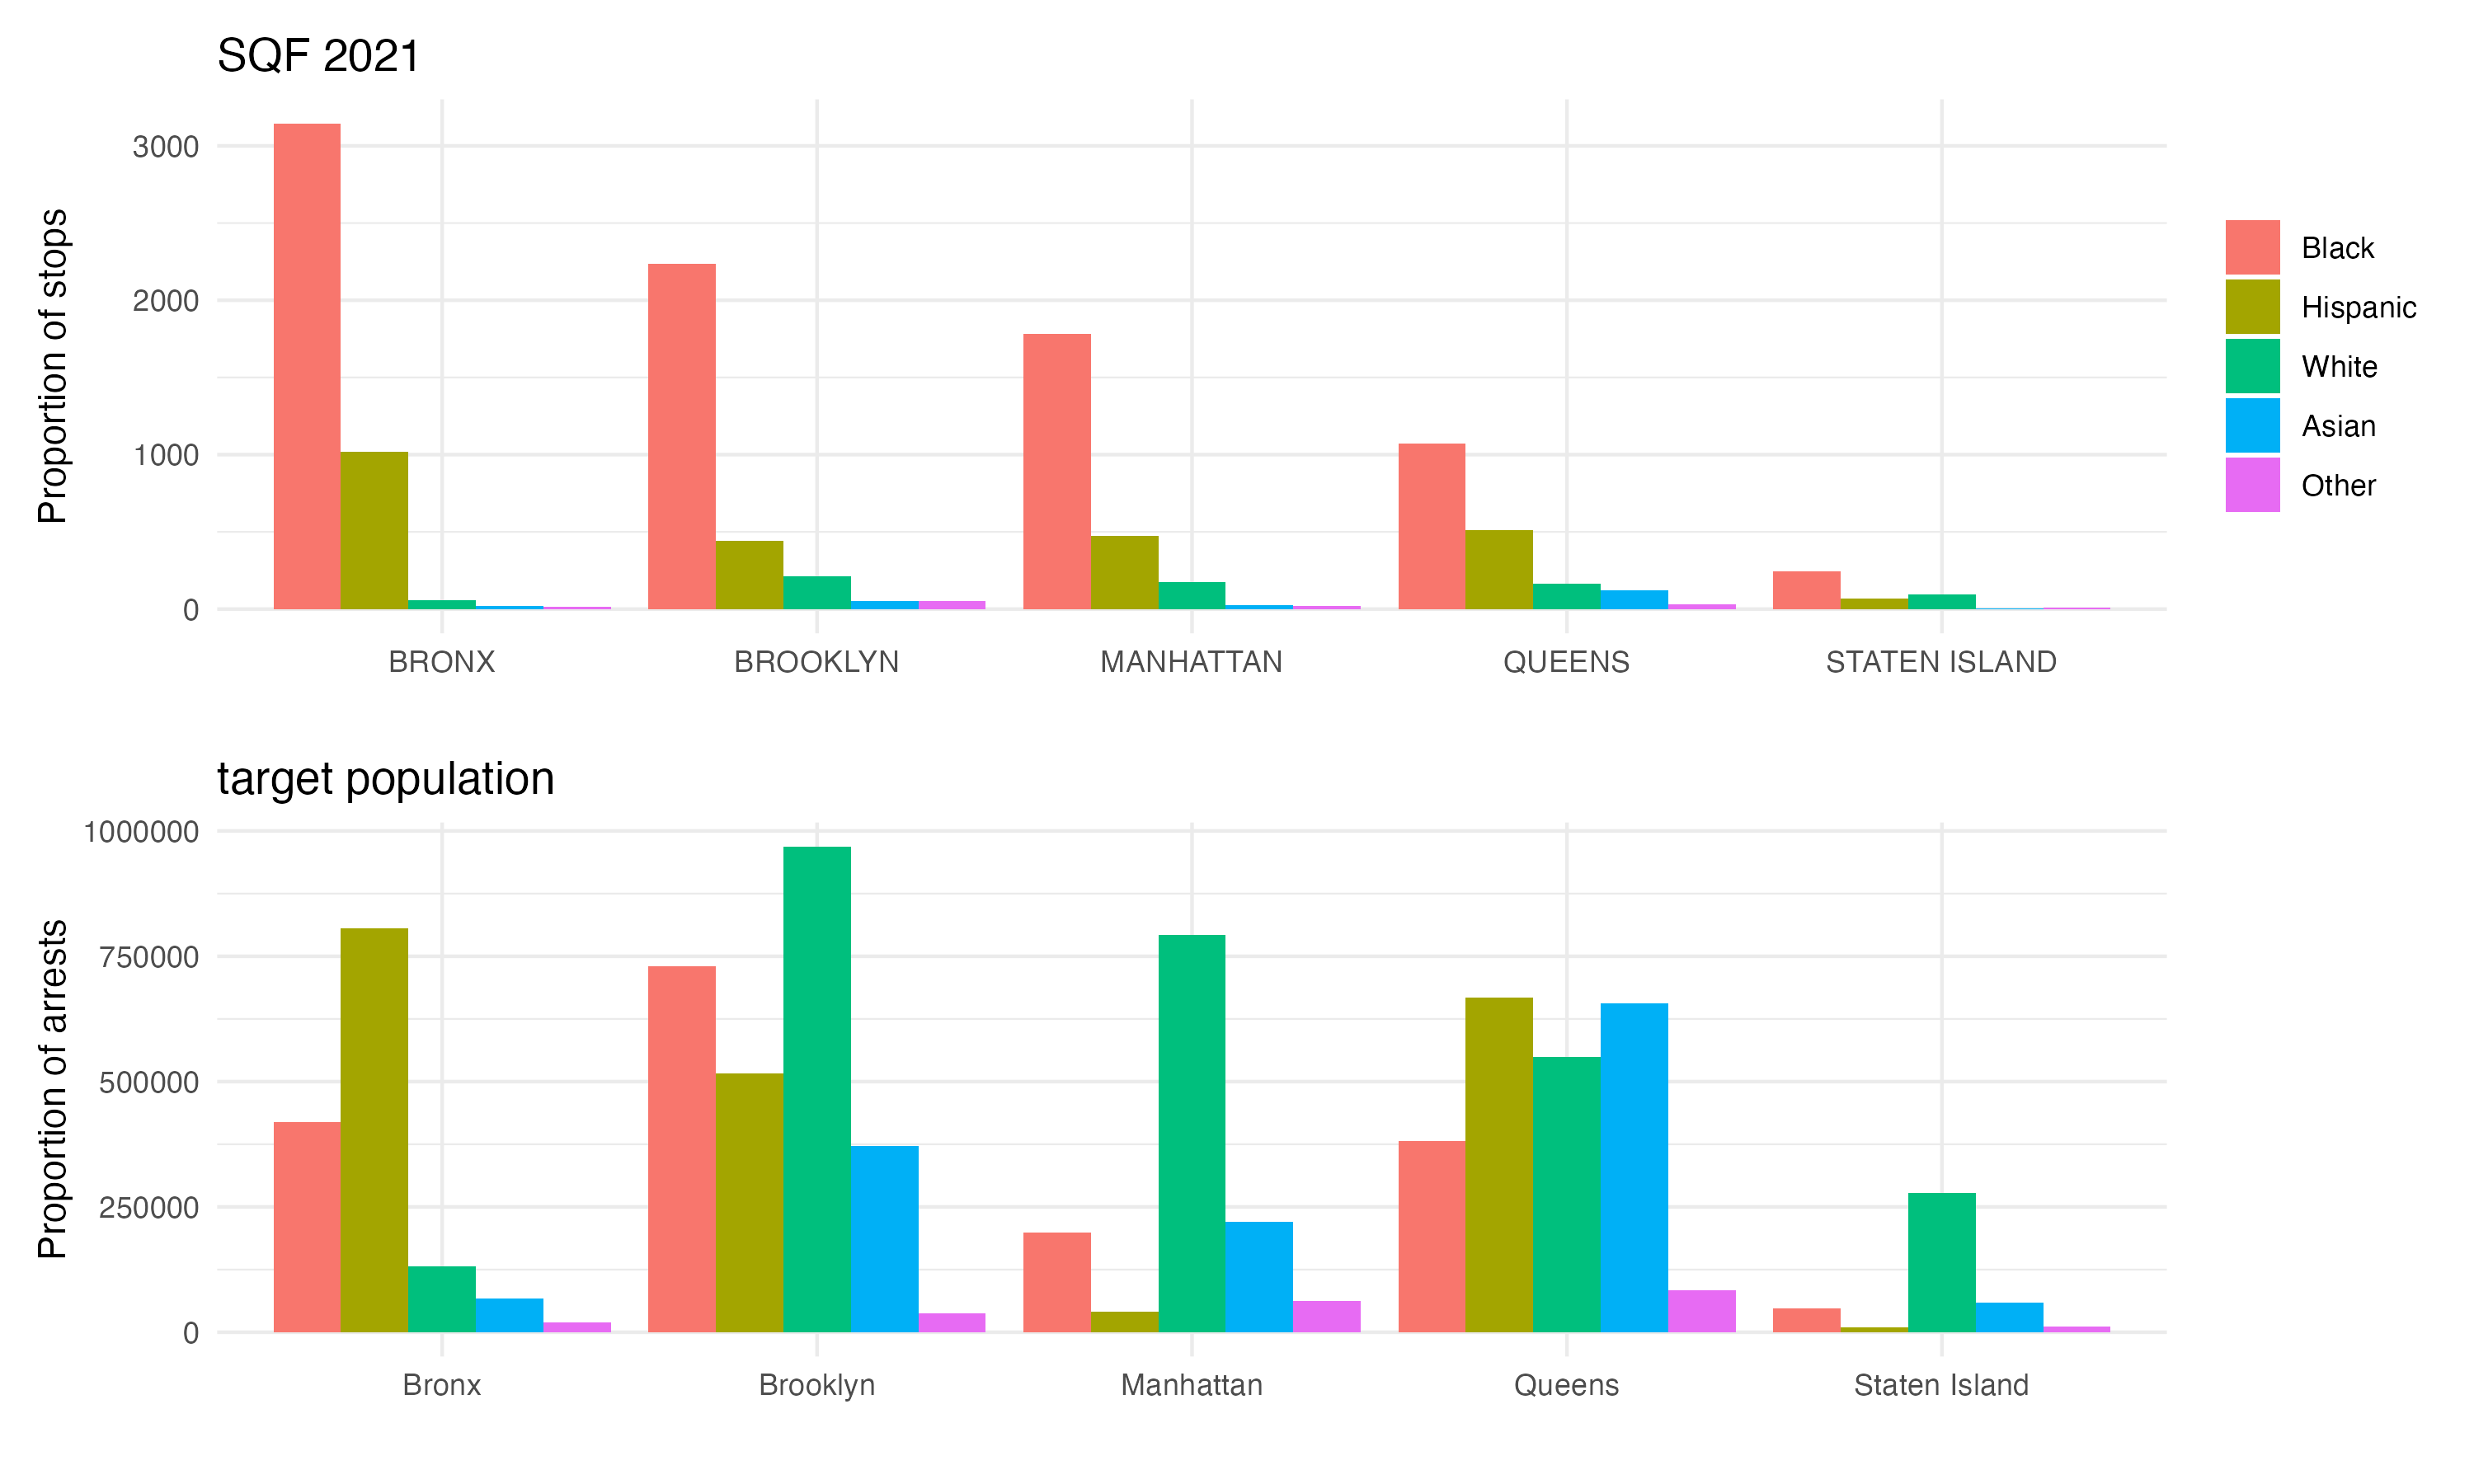
\includegraphics[width=0.7\textwidth]{../figures/sqf_case_study_plot11.png}
%     \caption {Distribution of race by borough in the SQF data (top) and NYC as a whole (bottom).}
%     \label{fig:borough_race_distribution}
% \end{figure}


\begin{landscape} % Rotates this section
    \subsection{Different approaches to fairness in SQF}

    Before going into detail about a specific study, we provide an overview of the different approaches to fairness in the SQF data.

    \begin{table}[h]
        \centering
        \renewcommand{\arraystretch}{1.2}
        \begin{tabular}{|p{3.5cm}|p{4.5cm}|p{3.5cm}|p{4cm}|p{4.5cm}|}
            \hline
            \textbf{Authors} & \textbf{Task} & \textbf{Model} & \textbf{Fairness Metric} & \textbf{Results} \\
            \hline
            \cite{kallus2018} 
            & Predict prob. of innocence (no weapon) 
            & Logistic Regression 
            & Equal Opportunity, Equalized Odds 
            & Bias against (Black) Hispanic individuals \\ 
            \hline
            \cite{RambachanBBOEFW} 
            & Task 1: Possession of contraband
            & Logistic Regression 
            & No explicit fairness metric; evaluate prediction function properties 
            & No disc. PoC\\
            \hline
            \cite{Badr2022DTFANSP} 
            & Predict probability of arrest 
            & Logistic Regression, Random Forest, XGBoost, GNB, SVC 
            & Balanced Accuracy, Stat. Parity, Equal Opportunity, Disparate Impact, Theil Index 
            & No disc. PoC \\ 
            \hline
            \cite{Khademi2019FADMELC} 
            & Predict probability of arrest 
            & Weighted regression models
            & FACE causal fairness (group), FACT fairness (individual) 
            & No group disc. PoC, but individual disc. PoC \\ 
            \hline
            \cite{goel2016} 
            & Predict possession of weapon 
            & (Penalized) Logistic Regression 
            & No explicit fairness metric; group-wise hit rates 
            & Black and Hispanic disproportionately involved in low-risk stops \\ 
            \hline
        \end{tabular}
        \caption{Summary of SQF-related Fairness Studies}
        \label{tab:sqf_summary}
  \end{table}
\end{landscape} % End rotation



\subsection{Sources of bias in the SQF data}
One of the main difficulties that come with the NYPD's data is that, when asking whether stop-and-frisk as a policing strategy is fair, one can come up with various tasks to try to answer this question. Only some of them are suitable to make conclusions about the fairness of the stop-and-frisk policy as a whole. As \cite{Badr2022DTFANSP} we trained a classifier to predict arrest and used group metrics to assess fairness. Given that both, the 2011 and 2023 regular RF classifier, performed well on the gorup metrics, but the stop-and-frisk practice was officially declared unconstitutional for 2011, fairness measured with these metrics for this classification task is not a good indicator for the fairness of the policy as a whole.\\
To answer the question of fairness in Stop-and-Frisk other studies take a step back and identify a problem with how the data is generated. They formalize and acknowledge that the discrimination in SQF does not lie in the outcome of the stop but the decision to stop someone in the first place.\\

\subsubsection*{Residual unfairness - problem setting}
In their paper "Residual Unfairness" \cite{kallus2018} conceptualize the problem as shown in \autoref{fig:selection_bias}.
We define a person by their sensitive feature (A) and non-sensitive features (X). For each person in the population of interest a police officer decides whether to stop them or not. This is the first potential source of bias. In the SQF context we can imagine that the police is generally more suspicious towards PoC than white people. Alternatively, we can imagine that they are stopping anyone more likely in high crime areas which happen to be correlated with low-income neighbourhoods which are mostly populated by PoC. \\
Based on this biased decision policy, individuals are either included in the sample or excluded from it $Z \in \{0,1\}$.  Naturally, we can only know the outcome $Y \in \{0, 1\}$ of a stop for the people who were stopped.
\cite{kallus2018} distinguish between target population and training population in such scenarios. The target population is the one on which we want to use the ADM on while the training population are the observations the biased decision policy chose to include in the sample and on which the algorithm is trained. The indicator $T \in \{0, 1\}$ tell us whether a person belongs to the target population. If $T = 1$ constantly, it means that the algorithm should be deployed for the entire population of NYC.\\
At this point, we refer back to \autoref{fig:race_distributions}. It shows a clear difference between the racial distribution in the SQF data and the city as a whole. In terms of race, the sample is clearly not representative for NYC. At the same time the estimated borough-specific crime rates also differ from the distribution of stops per borough as seen in \autoref{fig:nyc_pop_crimerates_stops_comparison}. \\

\begin{figure}
    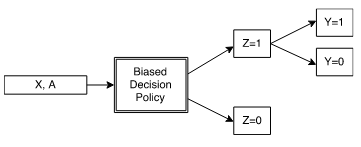
\includegraphics[width=0.7\textwidth]{../figures/selection_bias.png}
    \caption{Selection bias in the SQF data.}
    \label{fig:selection_bias}
\end{figure}

It is unclear whether a biased selection mechanism of such sort, can be captured by group metrics. They work with the joint distribution of $Y, A, \hat{Y}$ and do not take any additional information into account \footnote{There are variations of group metrics that allow for non-sensitive attributes $X$ to be considered as well when assessing fairness. An example is conditional statistical parity \cite{verma2018}.} . When we rely on the true label $Y$ to detect unfairness but the true label itself is not reliable (not generated via an objective truth), then the group metrics cannot show this mechanism (\cite{castelnovo2022}). Most group metrics offer a rather isolated view on fairness and qunatify differences in algorithmic predictions between groups rather than measuring the fairness of a whole situation.\\
On top of this, the mechanisms behind the selection bias in SQF is twisted in the sense that the historically discriminated group is \textit{more present} in the data. Often the situation is that disadvantaged groups form underrepresented minorities, thus the algorithm oversees them and performs worse on them. In the SQF data, however, the algorithm has plenty of observations from PoC to learn from and less from white people. More training data leads to better algorithmic performance and could explain why the classifier in chapter 5 performed mostly better for PoC.

\subsubsection*{Residual Unfairness - task and methods}
Before an officer stops a person, they need to have a suspicion about what the person did wrong. The suspected crime is recorded in the SQF data. The most common suspicion is the illegal possession of a weapon. \cite{kallus2018} limit themselves to only the stops where the suspected crime of the illegal possession of a weapon and the goal then becomes to predict the possession of a weapon. We refer to \cite{goel2016} for the detailed reasoning behind this approach.
Note that this is different to \cite{Badr2022DTFANSP} and our analysis, where the arrest is defined as the target variable.\\

\cite{kallus2018} train a logistic regression classifier and measure fairness in terms of equalized odds and equal opportunity. They find that non-white individuals are more often wrongly accused of possessing a weapon than white individuals. They apply a post-processing technique which assigns group specific thresholds to equalize the false negative rates/true positive rates (and the false positive rates/true negative rates in case of equalized odds) (\cite{hardt2016}).
After this fairness intervention the error rates are equal between groups when tested on the data the algorithm was trained on. However, when they claim that when the fairness-adjusted algorithm would be deployed on the population of NYC as a whole, racial discrimination against the historically discriminated persists. They do not test their dataset on actual new data from citizens but they design a way to estimate the error rates that would occur when the algorithm is deployed on the target population. They call the unfairness that comes from switching from training population to target population \textbf{residual unfairness} and identify it when training a classifier to predict the possession of a weapon on SQF data.\\
Here I would need to compare the results of one of the fairness classifiers (probably the EoD post-processing) and compare it to the estimated error rates. Does the classifier inherent the same tendencies?

\subsubsection*{Bias in, bias out? - problem setting}

% mathematical definitions I really need to get the point across
% - population as tupel of random variables (X, U, A, Y)
% - taste-based discriminator https://link.springer.com/referenceworkentry/10.1007/978-981-33-4016-9_1-1
Another perspective is offered by \cite{RambachanBBOEFW}
While the main message of \cite{kallus2018} is that even fairness adjusted classifiers exhibit the "bias in, bias out" mechanism \cite{RambachanBBOEFW} argue that is depends on the chosen classification task.

% problem setting, intro of selection bias
Similar to \cite{kallus2018} they are interested in whether a person carries a contraband. The paper assumes the police is a taste-based classifier against African-Americans. This means they hold some form of prejudice against the group of African-Americans that influences their decision to stop a member of this group. More precisely, they see the biased-decision policy in the decision to search someone; only on searched people a contraband can be found.\\

They formalise the problem as follows. For the decision-maker (the police) an individual is characterized by the random vector $(X, U, A)$, where X and A have the same meaning as in \cite{kallus2018}
and U is a set of unobserved features. These latent variables are unknown to the algorithm but are characteristics the police bases their decision to stop someone on. In the SQF context this could be the personal impression the officer got of a suspect which is not recorded and hard to measure.
In general, for searching any person, an officer incurs a cost $c > 0$. If they search an individual that truly carries a contraband, the officer receives a reward $b = 1$ \footnote{The reward can set to any number b > 0. We assume b = 1 as in \cite{RambachanBBOEFW} without loss of generality.}. In case of searching an innocent person $b = 0$.
For stopping African Americans the payoff an officer expects increases by $\tau > 0$ compared to stopping a white person. The total payoff for stopping an individual is given by:
$$Y + \tau * A - c$$
where $Y$ is the outcome of the search, $\tau$ is the discrimination parameter, $A \in \{0,1\}$, and $c > 0$ is the cost for searching a person.
Holding the costs $c$ and the outcome of the search $Y$ constant, searching an African American results in a higher payoff than searching a white person. The goal of the police is to maximize their payoff. Therefore, they search an individual according to the following threshold rule:
$$Z(X, U, R) = 1(E[Y|X, U, A] \ge c - \tau * A)$$
This means that the threshold for searching an African American is \textit{lower} than for a white person. Consequently, the police searches African Americans more leniently than white people.
In \cite{RambachanBBOEFW} the authors speak of "selective labels" where again the tupel $(Y, X, A, Z)$ is only available for $Z = 1$. We intentionally used $Z = 1$ to denote the search of an individual as it shows the parallel to the problem setting of \cite{kallus2018} depicted in \autoref{fig:selection_bias}. While in \cite{kallus2018} $Z = 1$ means a person was stopped and therefore included in the sample, in \cite{RambachanBBOEFW} $Z = 1$ means that the person was searched. In the latter study we restrict ourselves to an even smaller subset of the data but the selection bias mechanism remains the same.\\

\subsubsection*{Bias in, bias out? - task and methods}
Given this biased-selection mechanism that produces the training data, the authors distinguish between three classification scenarios.\\
In the first one, the goal is to predict the possession of a contraband, but the algorithm is trained on the biased sample that searched African Americans more leniently than white people. The disagreement again lies in that the algorithms tried to learn $Y$ from $Y | Z = 1$. In this case the algorithm will exhibit \textit{less} bias towards African Americans in the future. What happens is that as the police becomes more biased towards African Americans, they search them more leniently. This means that many innocent African Americans are included in the searched observations. Consequently, the model learns on average lower risk scores for African Americans. Essentially, the data for African Americans becomes more "noisy", more innocent people, without contraband are included, lowering the predicted probabilities for this group. The authors call this mechanism \textbf{bias reversal}.

% In their second classification task the idea is to train an algorithm to predict whether to search someone in the first place. Now the search becomes the target and here bias inheritance is observed. The same goes for a two stage classification ask that first predicts whether to search and then whether the individual carries a contraband if they were predicted as searched. What happens here is that as more of the stopped African Americans are also searched, the algorithm learns to associate search with more with African Americans than with white people and thus in the future also predicts higher probabilities for a search for African Americans. This is the \textbf{bias inheritance} mechanism.
% We can see parallels to this paper to our own case study in the sense that, PoC indeed have lower risk scores (density plot) and are relatively speaking less often predicted as arrested as white individuals.


\subsubsection*{Fairness through the lense of causality - problem setting}
Another paper from the field of fairML by \cite{Khademi2019FADMELC} approached the fairness problem in the SQF data from a causal perspective. As in our case study in section 4 they are interested in whether the decision to arrest someone after they have been stopped is discriminatory with respect to race, while they limit their comparison to Black-Hispanic and White men. They formalize the decision for an arrest made by the officer as a decision function $h: X x A \rightarrow Y$ and estimate the causal effect of race on the outcome from the data. For this they define two causal fairness metrics.
They write $Y_i^{(a)}$ and $Y_i^{(a')}$ for the outcomes of an observation $i$ when the sensitive attribute $A$ is set to $a$ and $a'$ respectively. Hereby $A = a$ is the observed value of the sensitive attribute for this observation and $A = a'$ is the counterfactual value. In the case of binary PAs this simply means that the person switches group membership. This is relevant because for causal fairness we essentially ask what outcome would the person have had if they were in the other group.\\
% \begin{definition}
%     \textbf{Fair on Average Causal Effect (FACE).}  
%     A decision function \( h \) is said to be fair, on average over all individuals in the population, with respect to \( A \), if  
%     \[
%     E[Y_i^{(a)} - Y_i^{(a')}] = 0.
%     \]
% \end{definition}

% \begin{definition}
%     \textbf{Fair on Average Causal Effect on the Treated (FACT).}
%     A decision function \( h \) is said to be fair with respect to \( A \), on average over individuals with the same value of \( A \), if  
%     \[
%     E[Y_i^{(a)} - Y_i^{(a')} \mid A_i = a] = 0.
%     \]
% \end{definition}

In words, FACE measure the difference between the true prediction and the counterfactual prediction for each data point and averages over these differences. However, in the most extreme case it could happen that $A = black$ were predicted as positive and their counterfactual parts $A = whitee'$ are predicted as negative - so there was a counterfactual switch in predictions. The switch works the other way around for the pairs of (actual white, counterfactual black). This has the consequence that all black individuals get a difference of 1 and all white ones a difference of -1. Taking the average this equalizes and hides the systematic bias.
This cannot happen with the second definition as we here condition on each group. Averaging out of causal discrimination can theoretically only happen within a group but not between groups anymore. Observational data of course does not contain the information needed for the estimation of their fairness definitions. They use Probability Weighting to estimate FACE and matching to estimate FACT. We refer to \cite{Khademi2019FADMELC} for the details.\\
To their own surprise, with FACT they find no racial discrimination against Black-Hispanic males, while FACE estimates that Black-Hispanic men are on average more likely to be arrested than white men.



% Overview of SQF studies
% Title: Residual unfairness in Fair Machine Learning from Prejudice Data
% Use of SQF:
% - task: predict probability of innocence (no weapon)
% - model: logistic regression
% - fairness: equal opportunity, equalized odds
% - results: classifier biased towards (Black) Hispanic individuals
% - key concepts: residual unfairness; estimation of error rates in target population via reweighing technique

% Title: Bias in Bias out? Evluating the Folk Wisdom
% Use of SQF:
% - task 1: predict probability of possession of contraband
% - task 2: predict probability of being searched
% - task 3: searched; if searched contraband (two-staged)
% - fairness: no explicit fairness metric; instead properties of the prediction function
% - model: logistic regression
% result: task 1 no discrimination against PoC, task 2 and task 3 discrimination against PoC
% key concepts: bias reversal, bias inheritance

% Title: Data Transparency and Fairness Analysis of the NYPD Stop-and-Frisk Program
% Use of SQF:
% - task: predict probability of arrest
% - model: Logistic Regression, Random Forest, XG Boost, GNB, SVC
%- fairness: Balanced Accuracy, Statistical Parity, Equal Opportunity, Disparate Impact, Avg. Odds Difference, Theil Index
% - results: no discrimination against PoC

% Title: Fairness in Algorithmic Decision Making: An Excursion Through the Lens of Causality
% Use of SQF:
% - task: predict probability of arrest
% - model: weighted regression models (FACE, FACT)
% - fairness: FACE causal group fairness, FACT causal individual fairness
% - results: no group discrimination against PoC, but individual discrimination against PoC
% - key concepts: fair on average causal effect (FACE), f air on average causal effect on the treated (FACT)

% Title: PRECINCT OR PREJUDICE? UNDERSTANDING RACIAL DISPARITIES IN NEW YORK CITY’S STOP-AND-FRISK POLICY
% Use of SQF:
% - task: predict probability possession of weapon
% - model: (penalized) logistic regression
% - fairness: no explicit fairness metric; group-wise hit rates
% - results: Black and Hispanic disproportionally involved in low-risk stops

% formal problem setting
% The selection bias we face means that we only have knowledge about $X, A, Y | Z = 1$ while we do not know $X, A, Y | Z = 0$. All information about the stop, the demographic details of the person and the outcome which serve as training label for an algorithm are only observed for stopped individuals.

% % Fairness definition
% The paper defines fairness via equal opportunity. Equal opportunity demands that the true positive rates across groups are equal, so that truly arrested individuals are predicted as such. In our case, in which a positive prediction $\hat{Y} = 1$ is undesirable it makes more sense to look at the false positive rates (or equivilantely at the true negative rates) and define fairness via predictive equality, i.e. $P(\hat{Y} = 1 | Y = 0, A = a) = P(\hat{Y} = 1 | Y = 0, A = b)$ or $P(\hat{Y} = 0 | Y = 0, A = a) = P(\hat{Y} = 0 | Y = 0, A = b)$.
% The paper looks at a thresholding classifier, if the prediction score exceeds a certain threshold the positive value for the target is predicted.
% This allows us express the false positive rate and the true negative rate of a group $a$ with respect to an event $E$ via the cummulative distibution function. $F_a^E = P(\hat{R} \leq \theta | Y = 1, A = a, E)$. Note that we condition on the truly negative subject in the sample. In the SQF case this would mean that we only look at people that were innocent, so not arrested.
% The truly arrested that have a predicted probability $\hat{R} \leq \theta$ are wrongly classified as not-arrested, while the ones for whom $\hat{R} > \theta$ are correctly classified as arrested. $F_a^Z$ gives us nothing other than the false negative rate in the training population and $F_a^T$ is the false negative rate in the target population.
% When we want to define a predictive equality classifier on the training population we require $F_a^Z(\theta_a) = F_b^Z(\theta_b)$ to hold. 

% % Definition of fair classifier 
% An optimal derived predictive equality classifier can then be defined as $\hat{Y} = I(\hat{R} > \theta_A)$ and $F_a^Z(\theta_a) = F_b^Z(\theta_b)$ for all groups a,b. In words, the classifier predicts the positive (undesirable)  outcome with a group-specific threshold for each member of the group while this group specific threshold is set in such a way that predictive equality on the training data is fulfilled. We will not go into detail of how one finds such a classifier but refer to \cite{hardt2016} who propose a post-processing method to derive the optimal thresholds for each group. 

% % Definition of unfairness inequity of predictive equality
% With the definition of fairness as predictive equality (equal tnr/fpr across groups) we can in turn define unfairness as nothing other than the difference in true negative rates between groups, i.e. \(\epsilon_{a,b}^E = P(\hat{Y} = 0 | Y = 0, A = a, E) - P(\hat{Y} = 0 | Y = 0, A = b, E)\) and call this inequity of predictive equality. $\epsilon_{a,b}^{T=1} > 0$ shows discrimination against group b, since this means that the true negative rate for group b is lower than for group a.
% When we construct an equal opportunity classifier (via some fairness intervention) then $\epsilon_{a,b}^{Z=1} = 0$ holds for this classifier. This also means that any unfairness that might show in the target population cannot be explained via existing ineuqities between groups in the training population but via existing differences in the training and the target population. So it is unfairness that gets introduced when we try to generalize our algorithm to the population it was not trained on. \cite{kallus2018} call this residual unfairness, since this is unfairness remaining event after fairness adjustments.

% % Scenarios of discrimination
% \subsubsection*{Strong disparate benefit of the doubt}
% To fully understand the results of the paper, we additionally introduce the concept of stochastic dominance, originating from decision theory. Let $F, G$ be two cummulative distribution functions. Then $G$ first order stochastically dominates $F \preceq G$ when $F(\theta) \geq G(\theta)$ $\forall\theta$. Recall that G and F are cumulative distribution functions. So first order stochastic dominance of G over F, smaller values of G for each input value $\theta$, that the population described by the CDF of G consistently has higher probability values than population F. Their probability mass is concentrated towards the higher input values thus the cummulative distribution function is small for small input values.
% Equipped with these definitions the paper constructs difference scenarios of (un)fairness. The bottom line is always that equal opportunity in the training population does not guarantee equal opportunity in the target population. We will introduce the one scenario mathemtically aligning the statements of the paper with the sqf scenario and will only conceptually explain the oterh scenarios which are extensions of the first one.

% % Scenario 1: Strong disparat benefit of the doubt (Prop. 2)
% We assume the following:
% $F_a^{Z=1} \succeq F_a^{T=1} and F_b^{Z=1} \preceq F_b^{T=1}$ and at least one of the equalities does not hold (either $F_a^{Z=1} \ne F_a^{T=1}$ or $F_b^{Z=1} \ne F_b^{T=1}$ or both).
% Then every derived equal opportunity classifier has nonnegative inequity of predictive equality for group b relative to group a $\epsilon_{a,b}^{T=1} \geq 0$ and at least one derived equal opportunity classifier will have a strictly positive inequity of predictive equality disadvantaging group b relative to group a $\epsilon_{a,b}^{T=1} > 0$.

% In words this means that for group a in the training population we have way more people with high scores (propbabilities of getting positive (undesirable) prediction) than in group a of the target population.
% So group a members were stopped very carefully. For group b members the opposite is true. In the train population of group b, there are many more people with low risk scores than there are in the target population of group b. This means group b members were stopped very leniently. 
% This aligns with the fact that the sqf data records considerably more stops for black people than white people. In this case the propositions of the paper will show us again that even after adjusting for equal error rates, the classifier will disadvantage group b when applied to the target population.
% The results of the paper would then say that adjusting a classifier for predictive equality, so equal false positive rates across groups, is not enough to ensure fairness on a whole and in future application. 

% % Extentions of scenario 1
% The paper admits that the assumptions are strict and in reality unlikeliky to be met. The assumptions would mean that the police is so biased against group b members that the proportion of low-risk group b members among stopped individuals is higher than the proportion of low-risk gorup b members in the general population. This would require a very unreasonable stopping policy.
% Therefore in the propositions that follow they weaken the assumptions. They allow that the stochastic dominance works in the same direction for both groups but the difference in training and target population for group b is so much more different than for group a that discrimination persists.
% Recall that the fairness definition of the paper is based on true positive rates and they are especially interested in the post-processing method by Hardt et al. The method takes as input the error rates of a classifier (e.g. the false positive and true positve error rates) in order to find group-specific thresholds that equalise these error rates across groups.
% If we now put in the "wrong" error rates, the error rates of the training population, which, however, are nto representative for the target population due to selection bias, we estimate the wrond thresholds. Therefore Kallus and Zhou offer a way to estimate the error rates in the target population based on training data and some additional information.
% These "corrected" error rates can then be used to create fairness interventions that will also spill over to the target population. Their approach is interesting and they use it on the SQF data themselves, but it is also very tailored towards error-rate-based group metrics and is mostly useful when the fairness method relies on the error rates, such as the thresholding by Hardt et al. When the fairness methods does not take error rates as an input, there is little use in estimating them for the target population.
% Though it could be interesting regardless, to get picture for how the algortihm could generalise.

% As the fairness audit in the previous chapter showed little disparities, we only take their method to estiamte the generalisation of the algorithm.
% We match the target population to the training population via borough.


% Things I have to introduce when I want to presente the math of the paper (e.g.Preposition 2)
% - Stochastic dominance
% - derived equal opportunity classifier
% - inequity of opportunity (epsilon)
% - Fairness defintion (equal tnr; predictive equality)